\subsection{CRISAM}
\subsubsection{Einleitung}

CRISAM (Corporate Risk Security Application Method) wurde von der Firma Calpana Business Consulting gmbh als Srtandard im Risikomanagement entwickelt. CRISAM® als Risikomanagement Methode folgt einem sechsstufigen Vorgehensmodell (gemäß ISO 31000). Unser Ziele mit der CRISAM® Risikomanagement Methode sind  es,  das komplexe Thema „Risiko“ einfach handhabbar zu machen, Risiken aus der Bauchhöhle herauszuholen und präzise bewerten zu können,  Chancen und Risiken im Unternehmen ganzheitlich und  wertorientiert darzustellen sowie Bewertungen und daraus resultierende Konsequenzen nachvollziehbar zu machen.
\\

Zu sehen ist die Risikomanagement Methode mit ihrem sechsstufigen Vorgehensmodell; Bild ~\ref{fig:bsp}

\begin{figure}[htbp]
\centering
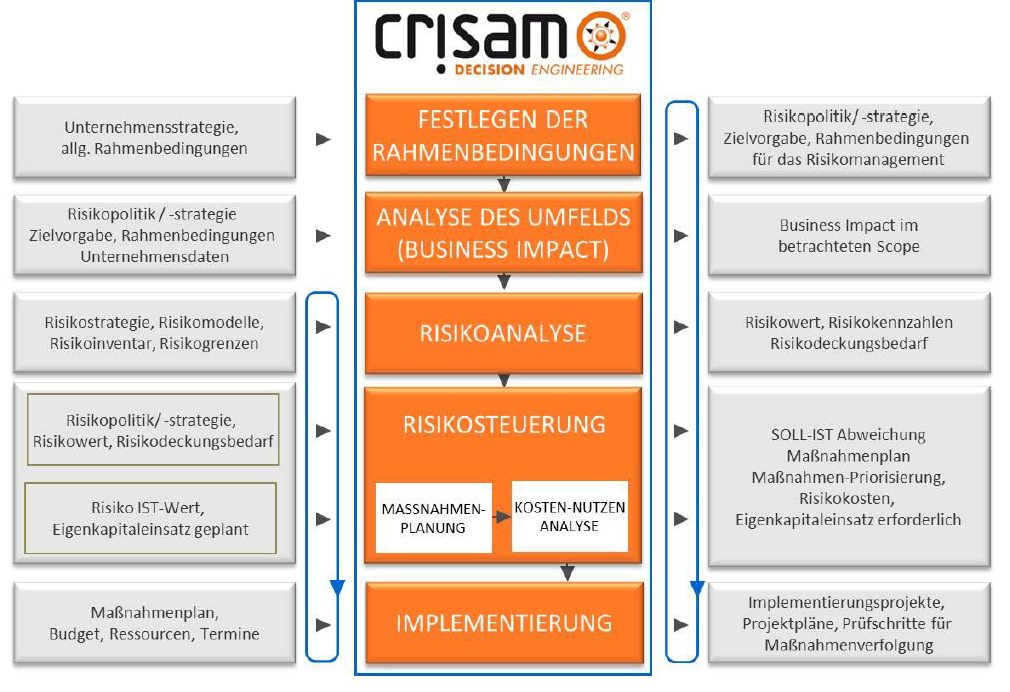
\includegraphics[scale =0.5 ]{images/Vorgehensmodell}
\caption{Crisam Vorgehensmodell}
\label{fig:bsp}
\end{figure}


	
\subsubsection {Stufe 1: Risikopolitik}
In Rahmen der Stufe 1: Risikopolitik wird ein IT-Security Leitbild, in dem die grundsätzliche Unternehmenskultur zum Thema IT-Security bzw. Grundsätze in den damit verbundenen Vorgehensweisen aus Sicht des Vorstandes oder der Geschäftsleitung festgelegt sind, erstellt. Folgende Themen werden behandelt:\\

- Zielsetzung und Strategie (Definition des Nutzens für den Kunden, das Unternehmen und die Mitarbeiter).

- Definition der Randbedingungen bzw. Relevanz von Daten und Informationen.

- Festlegen von Verantwortlichkeiten (Prozess- und Informationseigentümer).

- Festlegen einer Qualitätskennzahl an der sich das Risikomanagement als Sollwert zu orientieren hat.

- Einbettung des Risikomanagement und Sicherheitsmanagement Prozesses im Unter-nehmen.
\\
\\
Nutzen:

- Sicherung des Projekterfolges durch eine klare Vorgabe durch die Geschäftsleitung.

- Die IT-Sicherheitspolitik ist eine Dokumentation der Sollvorgabe für den Risikomanagement- bzw. Sicherheitsmanagement Prozess, die als Richtlinie und Entscheidungsgrundlage unternehmensintern verwendet.

- In der Erarbeitung der Zielsetzung wird der Nutzen des durchzuführenden Projektes dargestellt, sodass dem Projektaufwand der Wert des Ergebnisses gegenübergestellt werden kann.

- Die IT-Sicherheitspolitik liefert auch den klaren Auftrag, den dargestellten Nutzen für Kunden, externe Partner, Mitarbeiter und das Unternehmen selbst umsetzen zu müssen.
\\
\\
Ergebnis:\\
Die IT-Sicherheitspolitik liefert auch den klaren Auftrag, den dargestellten Nutzen für Kunden, externe Partner, Mitarbeiter und das Unternehmen selbst umsetzen zu müssen.

\paragraph {Festlegen der Bedrohungsklassen}
Zur Bewertung der möglichen Bedrohungen wurden Bedrohungsklassen festgelegt. Zur genauen Definition der Bedrohungsklassen wurden für jede Klasse sowohl eine verbale Beschreibung als auch eine Zuordnung zur Schadenshöhe. Die Schadenshöhe wurde von der Geschäftsführung definiert. Die Bedrohungsklassen dienten als Grundlage für die Klassifizierung bei den einzelnen Auditterminen.
\paragraph {Bedrohungsklasse und Beschreibung der Bewertung der Schadenshöhe}
Unbedeutend (0) : Risiken sowohl für Daten als auch IT-Anwendungen sind für das Unternehmen nicht relevant.
\\Gering (g): Bedrohungen sowohl für Daten als auch IT-Anwendungen werden als gering bewertet.
\\Mittel (m): Bedrohungen sowohl für Daten als auch IT-Anwendungen werden als mittel bewertet.
\\Hoch (h): Bedrohungen sowohl für Daten als auch IT-Anwendungen sind sehr wesentlich. Sach-, Personen- als auch inmaterielle Schäadenkönnen nicht mehr zur Gänze mit Kapital kompensiert werden.
\\ Sehr hoch (s): Bedrohungen sowohl für Daten als auch IT-Anwendungen werden als sehr hoch bewertet. Sach-, Personen- als auch inmaterielle Schäadenkönnen nicht mehr zur Gänze mit Kapital kompensiert werden.
\paragraph{Strategie}
Welche Bedeutung hat das IT-Risikomanagement für das Unternehmen? 
Wie wird sichergestellt, dass die Ziele, die mit der Einführung eines IT-Risikomanagements angestrebt werden, auch erreicht werden?
\paragraph{Geltungsbereich}
-Wo gelten die Leitsätze der IT-Sicherheitspolitik? (Abgrenzung innerhalb der Unternehmenslandschaft)
\\-Welche Prozesse / Abteilungen sind betroffen?
\\-Wie wird mit Schnittstellen zu anderen internen sowie als auch externen Organisationseinheiten umgegangen?
\\- Konkrete Benennung der Schnittstellen.
\\- Darstellung in einem Organigramm.
\paragraph{Schulung}
- Wer ist für die Initiierung, die Koordination, den Inhalt, sowie für die Dokumentation der Schulungsmaßnahmen im Kontext mit IT- Risikomanagement zuständig?
\\- Wer ist für die Teilnahme an Schulungsmaßnahmen verantwortlich?
\\- Wann sollen Schulungsmaßnahmen durchgeführt werden?
\paragraph{Management von Sicherheitsvorfällen}
- Wie erfolgt der Umgang mit Sicherheitsvorfällen?
\\- Wie erfolgt die Berichterstattung?
\\- Wie die Dokumentation ?
\\- Welche Konsequenzen werden vorgesehen?
\newpage
\subsubsection {Stufe 2: Geltungsbereich}
Um mit der Stufe 2 beginnen zu können, sollte die CRISAM® Stufe 1 (Risikopolitik) mit folgen-den Ergebnissen abgeschlossen worden sein:\\
\\- Die Risikopolitik ist definiert.
\\- Das angestrebte Zielrating ist festgelegt.
\\- Die Geschäftsprozesse, die im Geltungsbereich untersucht werden sollen, sind festge-legt.
\\- Die Bedrohungsklassen sind für die betrachteten Kriterien definiert.\\
\\
Ziel der CRISAM® Stufe 2 (Geltungsbereich) ist die Bestimmung der Auswirkungen auf die Geschäftsprozesse des betrachteten Unternehmens bei Eintreten bestimmter Szenarien. Die Szenarien ergeben sich aufgrund der untersuchten Kriterien. Um beispielsweise IT-Risiken zu identifizieren, sind die Kriterien Verfügbarkeit, Vertraulichkeit und Integrität maßgeblich.\\
Die in dieser Stufe durchgeführte Tätigkeit entspricht der Schutzbedarfsfeststellung nach BSI-Standard 100-2 sowie der im Rahmen der ISO/IEC 27001:2005 geforderten Analyse des Business Impacts.\\
Die allgemeine Vorgehensweise der CRISAM® Stufe 2 gliedert sich in die nachfolgend angeführten Teilschritte.
\paragraph{Geltungsbereich schulen}
In diesem Teilschritt erhalten die mit der Durchführung der Interviews betrauten Personen das notwendige Rüstzeug für eine erfolgreiche Interviewdurchführung.
\paragraph{Interwierpartner festlegen}
In diesem Teilschritt werden die verantwortlichen Personen, mit denen die Interviews durchgeführt werden, festgelegt. Um einen effizienten Interviewverlauf zu gewährleisten, ist darauf zu achten, dass die ausgewählten Personen mit den entsprechenden Prozessen vertraut sind.
\paragraph{Ziel}
Das Ziel des Interviews besteht darin, mit dem Geschäftsprozess-Verantwortlichen zu bestimmen, wie der Prozess von der IT unterstützt wird und wie die Abhängigkeiten des Prozesses von einzelnen IT-Services sind. Damit eine entsprechende Verbindlichkeit gewährleistet ist, muss die ausgearbeitete Dokumentation des Interviews vom jeweiligen Geschäftsprozess-Verantwortlichen unterzeichnet werden.

\paragraph{Identifikation des Bedrohungspotencials der Risikokriterien in Bezug zum Gesamtprozess}
Zuerst wird der Gesamtprozess betrachtet, anschließend erfolgt die eigentliche Bewertung auf Basis der verwendeten IT-Services. Damit wird eine Kontroll- und Vergleichsmöglichkeit ermöglicht, weil die Einschätzungen die für den Gesamtprozess getroffen wurden, die Obergrenze darstellen und nicht von der Einschätzung einzelner Services überschritten werden dürfen.\\
\\Verfügbarkeit (Standardwert: 2 Tage)
\\-Was sind die Auswirkungen aus Sicht des Geschäftsprozesses auf das gesamte Unter-nehmen, wenn keine IT-Services verfügbar sind, z.B. zentraler Netzwerkausfall.\\
-Kann die Geschäftstätigkeit/Handlungsfähigkeit des Unternehmens trotz Gesamtausfall der IT-Services in irgendeiner Form aufrechterhalten werden?\\
\\Vertrauligkeit
\\-Was sind die Auswirkungen, falls kritische Daten nach außen gelangen/ veröffentlicht werden?
\\-Welcher eingetretene Schaden wird als der Worst Case gesehen?\\
\\Integrität
\\-Was sind die Auswirkungen, falls mit falschen oder unvollständigen Daten gearbeitet wird?
\\-Wie wird die Integrität der Daten sichergestellt (auch Schutz vor Datenverlust)?
\subsubsection{Stufe 3: Risikoanalyse}
Innerhalb dieser Stufe sollen konkrete Aktivitäten für die Umsetzung des IT-Risikomanagements im Unternehmen durchgeführt werden. Das Vorgehensmodell ist wie folgt aufgebaut.\\
\\Die Risikoanalyse erfolgt in zwei Teilschritten. Im ersten Teilschritt (Strukturanalyse) wird aus-gehend von den IT-Services die IT-Landschaft in ihre einzelnen Bestandteile zerlegt (=Risikoobjekte), im zweiten Teilschritt erfolgt dann die Bewertung dieser Risikoobjekte. Die Gesamtbewertung ergibt sich dann aus der Bewertung der einzelnen Risikoobjekte.
\paragraph{Wie ist die Struktur aufzubauen}
Die Struktur erfolgt immer als Baumstruktur, wobei in der obersten Verzweigungsebene (Wurzelknoten des Baumes) der Konzern und seine Töchter oder ähnlich Einheiten dargestellt wer-den. Hierfür stehen in CRISAM® sogenannte Container-Bausteine zur Verfügung (Container-Bausteine enthalten im Unterschied zu den übrigen Bausteinen keine Kontrollziele). Im Speziellen sind dies die Bausteine: Konzern und Unternehmen.

\begin{figure}[htbp]
	\centering
	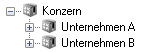
\includegraphics[scale =1 ]{images/Modellierung.png}
	\caption{Modellierung oberste Ebene}
	\label{fig:bsp}
\end{figure}
Nachdem im Rahmen der Stufe 2: Geltungsbereich, die zu betrachtenden Geschäftsprozesse oder Unternehmenseinheiten bestimmt wurden, müssen diese entsprechend im Baum modelliert werden. Hierzu stehen die folgenden Bausteine zur Verfügung: Geschäftsprozess, Kernprozess, Management-Prozess, Support-Prozess, Teilprozess, Aufgabe, Aktivität.
Folgende Abbildung soll einige mögliche Konstellationen zeigen. Die Modellierung dieser Teilstruktur kann in beliebiger Tiefe erfolgen. Schlussendlich soll die Modellierung auf dieser Ebene die Realität möglichst getreu abbilden.

\begin{figure}[htbp]
	\centering
	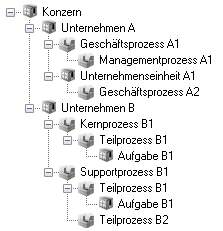
\includegraphics[scale =1 ]{images/weiterebenen.png}
	\caption{Modellierung weitere Ebenen}
	\label{fig:bsp}
\end{figure}

\paragraph{IT-Services}
Die in Stufe 2 definierten Business IT-Services bauen jeweils auf einem Technical IT-Service auf, der die entsprechende Applikation darstellt. Ein Technical IT-Service steht in Abhängigkeit zu der Applikation (z.B. Zeiterfassung-Applikation) und dem IT-System (z.B. Server004) auf dem diese betrieben wird. Dies wird in Abbildung 5 - Technical IT-Service Zeiterfassungs-Service dargestellt.
\newpage
\begin{figure}[htbp]
	\centering
	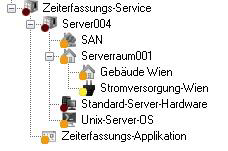
\includegraphics[scale =1 ]{images/Technical.png}
	\caption{Technical IT-Service Zeiterfassungs-Service}
	\label{fig:bsp}
\end{figure}
\paragraph{Modellierung der IT-Prozesse nach ITIL v2. COBIT bzw. ISO 27001}
In der folgenden Abbildung sind die Objekte „IT-Prozesse“, „IT-Prozesse Administrativ“, „IT-Prozesse Operativ“ und „IT-Prozesse Strategisch“ lediglich als Strukturelemente gedacht (dazu werden Container-Bausteine verwendet). Diese Anwendung von Objekten als Strukturelemente ist nicht zwingend notwendig, empfiehlt sich jedoch im Hinblick auf eine gute Übersichtlichkeit und optimale Auswertemöglichkeiten. Die Verwendung der untenstehenden Bausteine, ausgenommen „Langzeitarchivierung“ ist zwingend notwendig.
Um das Backup (allg. Konzept im Unternehmen) im Baum darzustellen, ist es mindestens erforderlich, ein darunterliegendes Datenträgerarchiv zu modellieren.
Soll die Langzeitarchivierung in die Risikobetrachtung mit aufgenommen werden, so ist auch hier mindestens die Modellierung eines darunter liegenden Datenträgerarchivs erforderlich.
\begin{figure}[htbp]
	\centering
	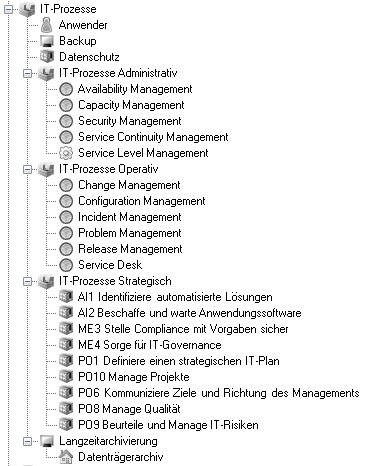
\includegraphics[scale =1 ]{images/prozesse.png}
	\caption{Modellierung IT-Prozesse}
	\label{fig:bsp}
\end{figure}
\paragraph{Modellierung eines Server-Systems}
Für das Objekt Server Betriebssystem kommen die Bausteine „Betriebssystem“.Für das Objekt „Server Hardware“ ist der Baustein „Server-Hardware“, für das Objekt „Serverraum“ ist der Baustein „Serverraum“, für das Objekt „Gebäude“ ist der Baustein „Gebäude“ und für das Objekt „Stromversorgung“ ist der Baustein „Stromversorgung“ zu verwenden.
\begin{figure}[htbp]
	\centering
	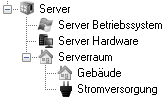
\includegraphics[scale =1 ]{images/server.png}
	\caption{Modellierung Server}
	\label{fig:bsp}
\end{figure}

\subsubsection{Stufe 4/5: Risikomanagement}
Im Rahmen der Stufe 4/5 Risikomanagement wird ein Maßnahmenkatalog zur Erreichung des angestrebten Sollzustands erarbeitet. Dazu sind folgende Schritte notwendig:\\\\
1. SOLL-IST Analyse aufgrund von Policy bzw. Geltungsbereich und Risikoanalyse: Ausge-hend von den definierten SOLL-Vorgaben aus der Policy und Geltungsbereich werden die wesentlichen Abweichungen zum ermittelten IST-Zustand aus der Risikoanalyse identifiziert und erklärt.\\
2. Verbesserungsvorschläge identifizieren: Ausgehend von den Ergebnissen der Risikoana-lyse werden die erforderlichen Verbesserungsvorschläge identifiziert.\\
3. Maßnahmen definieren: Auf Basis der Risikoanalyse werden die einzelnen Kontrollziele und die dazu identifizierten Verbesserungsvorschläge zu Maßnahmen zusammengefasst.

Ein Risiko besteht dann, wenn die Ist-Objekterfüllung negativ von der Soll-Objekterfüllung ab-weicht. Im Gegensatz dazu, bedeutet eine positive Abweichung, dass eine Chance besteht. Eine Chance bedeutet in diesem Zusammenhang bspw. Einsparung von Kosten oder etwa für künftige Herausforderungen entsprechend vorbereitet zu sein.
\paragraph{Soll - Ist Analyse}
Ein Risiko besteht dann, wenn die Ist-Objekterfüllung negativ von der Soll-Objekterfüllung ab-weicht. Im Gegensatz dazu, bedeutet eine positive Abweichung, dass eine Chance besteht. Eine Chance bedeutet in diesem Zusammenhang bspw. Einsparung von Kosten oder etwa für künftige Herausforderungen entsprechend vorbereitet zu sein.

\paragraph{Verbesserungsvorschläge identifizieren}
Verbesserungsvorschläge werden mit den folgenden Schritten identifiziert:\\
- Identifizierung der relevanten Kontrollziele mit Hilfe des GAP-Berichtes und den Kontrollzieldetails.
\\- Durch Vergleich der Ist-Erfüllung eines Kontrollzieles mit der vom System vorgeschlagenen Soll-Erfüllung können jene Kontrollziele bei denen Verbesserungsbedarf besteht identifiziert werden.
Anhand des Berichtes „GAP-Analyse“ lässt sich erkennen, welche Objekte näher betrachtet werden müssen, um entsprechende Verbesserungsvorschläge zu identifizieren.
\paragraph{Maßnahmen definieren}
Die zuvor identifizierten Kontrollziele mit den dazugehörigen Verbesserungsvorschlägen wer-den nun nach sinnvollen Kriterien zu Maßnahmen zusammengefasst. Diese Kriterien sind übli-cherweise inhaltlicher, technischer oder strategischer Natur. Technische Maßnahmen wären bspw. „Bauliche Maßnahmen“, „Release Management verbessern“, „Server Hardware verbes-sern“, etc.
Dazu ist es zuerst notwendig eine neue Maßnahme anzulegen (siehe Abbildung 6: Risikoma-nagement – Maßnahmen). Im nächsten Schritt werden die einzelnen Maßnahmen näher unter-sucht und hinsichtlich:\\
- Dringlichkeit,\\
- Kosten (grobe Kostenabschätzung),\\
- Kategorie (technisch, organisatorisch, rechtlich)
klassifiziert.
\subsubsection{Stufe 6: Implementierung}
Die Implementierung unterstützt das Unternehmen durch die Zusammenfassung von Maßnah-men zu Projekten, in welchen Ressourcen, Termine und budgetäre Belange festgehalten wer-den.
Dieses Dokument enthält Hinweise zum Teilschritt „Implementierung“ und beantwortet die Frage, wie das Zusammenfassen von Maßnahmen zu Implementierungen bzw. Projekten der IT Organisation behilflich ist.
\paragraph{Implementierung definieren}
Im Rahmen der Implementierung – der 6. Stufe des CRISAM Vorgehensmodells - werden die einzelnen Maßnahmen nach technologischer und organisatorischer Umsetzbarkeit bewertet und erforderliche Aktivitäten und Projekte initialisiert.
\paragraph{Zuordnung von Maßnahmen}
Schlussendlich sollen einer Implementierung Maßnahmen zugeordnet werden. Dies geschieht über den Reiter „Zugeordnete Maßnahmen“ – hier sind bereits zugeordnete Maßnahmen sichtbar – und der Funktion „Maßnahmen zuordnen“. Es werden alle zuvor angelegten Maßnahmen aufgelistet und über das Setzen des entsprechenden Häkchens und der Bestätigung über „Maß-nahmen zuordnen“ erfolgt die jeweilige Zuordnung.
\paragraph{Zusammenfassung}
Im CRISAM-TOOL wird ein Modell der IT-Infrastrukturen mit deren Ursache Wirkungsbeziehung abgebildet. Aufgrund dieser Abbildung in einem Fehlerbaum und der Risikoquantifizierung aller Risikoobjekte des Baumes, kann an der Wurzel des Baumes, dem Geschäftsprozess,das aggregierte Risiko abgelesen werden. Dem Wurzelwert wird im Rahmen der Risikopolitik, ein für das Unternehmen adäquates Restrisiko zugeordnet. Damit ist der „Risikoappetit“ bzw. das vom Unternehmen akzeptierte Restrisiko bestimmt.
CRISAM ermittelt jene Verbesserungspotenziale je IT-System, IT-Prozess bzw. je IT-Infrastruktur,
die für die Erreichung der Zielvorgabe erforderlich umzusetzen sind.
Werden Maßnahmen identifiziert, so können sie im Sinne einer „Was wäre wenn?“ Analyse auf Effizienz und Effektivität simuliert werden. Jede Investition kann im Kontext des aktuell gültigen Entscheidungsraumes begründet werden. Für eine spätere Validierung der Entscheidung kann die ursprünglich verwendete Umgebung wiederum zugrunde gelegt werden.
\\
\\
Aufgrund beschränkter Zugriffsrechte konnten gewisse Funktionen nicht ausgeführt werden, jedoch konnte die Erreichung der Ziele durch die Software nachvollzogen werden.
Die Lizenz kostet 20,000 Euro pro Jahr. BSI-Standard sind in CRISAM vorhanden. Dokumentation und Tutorials sind nur für Kunden vorhanden. 

\subsubsection{Bewertung}
\begin{table}[h]
%\centering
\begin{tabular}{|p{0.5\textwidth}|p{0.5\textwidth}|}
\hline 
Kriterium & Bewertung \\ 
\hline 
\textbf{GUI}& \\
\hline
Wizard & 7 \\
\hline 
Infrastrukturdarstellung & 10 \\
\hline 
Netzpläne & 3 \\
\hline 
Prozessflüsse & 5 \\
\hline 
Schnelles Einpflegen von Änderungen & 7 \\
\hline
\textbf{Objektrelationen} & \\
\hline 
Doppelseitige Verlinkungen & 0 \\
\hline 
Vererbung & 10 \\
\hline 
Gruppierungen & 8 \\
\hline 
\textbf{Funktionalität} & \\
\hline 
Aktuelle BSI-Standards & 10  \\
\hline  
Erweiterbarkeit der Klassifizierungen & 10 \\
\hline 
Individuelle Beschreibungen & 0 \\
\hline 
Sicherheitsverstöße markieren & 8  \\
\hline
Bewertung des Sicherheitsstatus & 10 \\
\hline
Export von Berichten & 0  \\
\hline
BSI-Toolimport & 10 \\
\hline
Sicherheit des Tools an sich & 10 \\
\hline
Risikobewertung & 0 \\
\hline
\textbf{System}&\\
\hline
Verteiltes Arbeiten & 10\\
\hline
Rechtevergabe & 10 \\
\hline
Kosten & 10 \\
\hline
Support & 8  \\
\hline
Zertifizierung & 10 \\
\hline
Dokumentation & 5  \\
\hline
Marktpräsenz & 10  \\
\hline
Spezielle Zielgruppe & 4  \\
\hline
Pflege/Weiterentwicklung & 0 \\
\hline
\multicolumn{2}{c}{}\\
\hline
\textbf{Gesamt} & \\
\hline
Hochschuleinsatz & 71\%\\
\hline
Lehre & 70\%\\
\hline

\end{tabular} 
\caption{Bewertung: Crisam}
\label{tab:Berwertung Crisam}
\end{table}
Die Auswertungstabelle zeigt die von mir bewerteten Kriterien und die daraus resultieren Daten für die Hochschule und die Lehre. 
Die Kriterien wurden untergliedert in Gruppen nach GUI, Objekrelationen, Funktionalität und System.
\\
Bei GUI wurden die Bewertung von 3 bis 10 Punkte vorgenommen. 
Die niedrigste Punktvergabe hat Netzpläne, weil sie im Programm nicht ausführlich vorkommen.
\\
Die Infrastrukturdarstellung wurde mit 10 Punkte bewertet, weil verschiedene Darstellungen möglich sind.
In der Gruppe der Objektrelationen wurde die Vererbung mit 10 Punkten bewertet, da sie sehr gut vorhanden sind.
\\
In der Funktionalitätsgruppe sind aktuelle BSI-Standards, Erweiterbarkeit der Klassifizierungen, Bewertung des Sicherheitsstatus, BSI-Toolimport und Sicherheit des Tools mit 10 Punkten bewertet, weil sie im Programm sichtbar sind.
Bei der letzten Gruppenabteilung sind die Dokumentation und spezielle Zielgruppen am schlechtesten bewertet, da Tutorials und Dokumentation zur Nutzung des Tool nicht vorhanden waren. Deshalb ist das Tool nicht für die Ausbildung und zum Zweck des Studiums geeignet, weil man es nicht umfangreich testen konnte.
\\
\\
Die Ergebnisse zeigen sowohl für die Hochschule als auch für die Lehre etwa 70 Prozent, das bedeutet das Crisam ein geeignete GS-Tool ist.